% Created 2016-09-05 lun 11:27
\documentclass[11pt]{article}
\usepackage[utf8]{inputenc}
\usepackage[T1]{fontenc}
\usepackage{fixltx2e}
\usepackage{graphicx}
\usepackage{grffile}
\usepackage{longtable}
\usepackage{wrapfig}
\usepackage{rotating}
\usepackage[normalem]{ulem}
\usepackage{amsmath}
\usepackage{textcomp}
\usepackage{amssymb}
\usepackage{capt-of}
\usepackage{hyperref}
\author{Tipos de Datos}
\date{\textit{<2016-08-29 lun>}}
\title{Conceptos Avanzados en Lenguajes de Programación}
\hypersetup{
 pdfauthor={Tipos de Datos},
 pdftitle={Conceptos Avanzados en Lenguajes de Programación},
 pdfkeywords={},
 pdfsubject={},
 pdfcreator={Emacs 24.5.1 (Org mode 8.3.2)}, 
 pdflang={English}}
\begin{document}

\maketitle
\tableofcontents


\section*{Introducción}
\label{sec:orgheadline49}

\subsection*{Tipos de Datos}
\label{sec:orgheadline7}
\begin{itemize}
\item Hemos desarrollado una noción intuitiva de tipo de dato; ¿Que hay
detras de la intuición?
\begin{itemize}
\item Conjunto de valores de un "dominio" (la aproximación funcional)
\item Estructura interna de un manojo de datos, descripto al nivel de un
conjunto pequeño de tipos fundamentales (aproximación estructural)
\item Clase de equivalencia de objetos (aproximación del implementador)
\item Conjunto de operaciones bien-definidas que pueden ser aplicadas a
objetos de ese tipo (aproximación de abstracción)
\end{itemize}
\end{itemize}

\subsubsection*{Tipos de Datos}
\label{sec:orgheadline1}
\begin{itemize}
\item Utilidad
\begin{itemize}
\item Contexto implícito
\item Chequeo de tipos
\begin{itemize}
\item Asegura que ciertas operaciones erróneas no ocurran
\item aunque no puede prevenir todas
\end{itemize}
\item polimorfismo surge cuando el compilador encuentra que no necesita saber ciertas cosas
\end{itemize}
\end{itemize}

\subsubsection*{Tipos de Datos}
\label{sec:orgheadline2}
\begin{itemize}
\item \textbf{Fuertemente Tipado} se ha vuelto un término popular
\begin{itemize}
\item como \emph{programación estructurada}
\item informalmente, significa que el lenguaje previene al programador
de aplicar operaciones a los datos que no son apropiados
\end{itemize}
\item \textbf{Tipado Estático} significa que el compilador puede realizar todos
los chequeos en tiempo de compilación.
\item Ejemplos
\begin{itemize}
\item Common Lisp is fuertemente tipado pero no \textbf{tipado estaticamente}
\item Ada es estáticamente tipado
\item Pascal es casi estáticamente tipado
\item Java es fuertemente tipado, con una mezcla no trivial de cosas que
pueden ser chequeadas estaticamente y cosas que tienen que ser
chequeadas dinámicamente.
\end{itemize}
\end{itemize}


\subsubsection*{Tipos de Datos}
\label{sec:orgheadline3}
\begin{itemize}
\item Simples
\begin{itemize}
\item Primitivos: integer, float, char, enum
\item Definidos por el Usuario
\end{itemize}
\item Compuestos
\begin{itemize}
\item Arreglos
\begin{itemize}
\item strings
\end{itemize}
\item Arreglos asociativos
\item Registros
\item Union
\item conjuntos
\item listas
\item punteros
\item archivos
\end{itemize}
\end{itemize}

\subsubsection*{Sistema de Tipos}
\label{sec:orgheadline4}
\begin{itemize}
\item Un \textbf{Sistema de Tipos} tiene reglas para
\begin{itemize}
\item equivalencia de tipos (¿cuándo los tipos de dos valores son el mismo?)
\item compatibilidad de tipos (¿cuándo puede el valor de un tipo A ser
usado en un contexto donde se espera el tipo B?)
\item inferencia de tipos (¿Cuál es el tipo de una expresión, dado el
tipo de los operandos?)
\end{itemize}
\end{itemize}

\subsubsection*{Chequeo de Tipos}
\label{sec:orgheadline5}
\begin{itemize}
\item Dos Aproximaciones: \emph{equivalencia estructural} y \emph{equivalencia por nombre}
\begin{itemize}
\item La equivalencia por nombre esta basado en las declaraciones
\item La equivalencia estructural esta basada en la noción de
significado detrás de esas declaraciones
\item Equivalencia por nombre es mas preferida hoy en dia.
\end{itemize}
\end{itemize}

\subsubsection*{Estructural vs. por Nombre}
\label{sec:orgheadline6}
\begin{itemize}
\item a veces es preferible estructural
\end{itemize}
\begin{verbatim}
TYPE stack_element = INTEGER; (* or whatever type the user prefers *) 
MODULE stack; 
IMPORT stack_element; 
EXPORT push, pop; 
...
PROCEDURE push(elem : stack_element); 
...
PROCEDURE pop() : stack_element; 
...
\end{verbatim}
\begin{itemize}
\item otras veces por nombre
\end{itemize}
\begin{verbatim}
TYPE celsius_temp = REAL; 
fahrenheit_temp = REAL; 
VAR c : celsius_temp; 
    f : fahrenheit_temp; 

BEGIN (* alias_types *)
    c := 100.0;
    f := c;                 (* this should probably be an error *)
\end{verbatim}

\subsection*{Chequeo de Tipos: Coerción}
\label{sec:orgheadline12}

\subsubsection*{Chequeo de Tipos: Coerción}
\label{sec:orgheadline8}
\begin{itemize}
\item Coerción
\begin{itemize}
\item Cuando una expresión es usada en un contexto donde un tipo
diferente se espera, uno normalmente obtiene un error.
\item Pero, y en esta situación?:
\end{itemize}
\end{itemize}
\begin{verbatim}
var a : integer; b, c : real;
...

c := a + b;
\end{verbatim}
\begin{itemize}
\item Muchos Lenguajes lo permiten.
\item Puede ser basado solo en los tipos de los operandos (Fortran)
\end{itemize}
\subsubsection*{Chequeo de Tipos: Coerción}
\label{sec:orgheadline9}
\begin{itemize}
\item Coerción
\begin{itemize}
\item \textbf{C} usa mucha coerción, pero con reglas simples:
\begin{itemize}
\item todos los \texttt{float}  en expresiones se vuelven \texttt{double}
\item \texttt{short} \texttt{int} y \texttt{char} se vuelven \texttt{int} en las expresiones
\item Si es necesario, la precisión es removida cuando se asigna a
lado izquierdo de la asignación.
\end{itemize}
\end{itemize}
\end{itemize}

\subsubsection*{Chequeo de Tipos: Coerción}
\label{sec:orgheadline10}
\begin{itemize}
\item De hecho, las reglas de coerción son una relajación del chequeo de tipos
\begin{itemize}
\item Nuevas opiniones lo consideran una mala idea
\item Lenguajes como Modula-2 y Ada no permiten coerción
\item C++, sin embargo lo usa en extremo
\end{itemize}
\end{itemize}

\subsubsection*{Chequeo de Tipos: Coerción}
\label{sec:orgheadline11}
\begin{itemize}
\item Es importante entender la diferencia entre:
\begin{itemize}
\item \textbf{Conversión de Tipos} que es \emph{explícito} y
\item \textbf{Coerción de Tipos} que es \emph{implícito}
\item para las conversiones a veces se usa la palabra \emph{cast} (por C)
\end{itemize}
\end{itemize}


\subsection*{Arreglos}
\label{sec:orgheadline30}
\begin{itemize}
\item Los Arreglos son el tipo compuesto mas importante en los lenguajes
de alto nivel. Es una agrupación de elementos (usualmente) homogeneos
 en la cual los elementos individuales son son
identificados por su posición en la agrupación relativo a su primer
elemento.
\end{itemize}

\subsubsection*{Cuestiones de Diseño de Arreglos}
\label{sec:orgheadline13}

\begin{itemize}
\item ¿Cuales tipos son legales para ser subíndices?
\item ¿Es chequeado que el subíndice cumpla el rango definido?
\item ¿Cuándo se liga el rango de subíndices?
\item ¿Cuándo tiene lugar el alojamiento de espacio?
\item ¿Cual es el número máximo de subíndices?
\item ¿Pueden los arreglos ser inicializados?
\item ¿Se pueden definir porciones (slices) de arreglos?
\end{itemize}

\subsubsection*{Accediendo a los elementos del Arreglo}
\label{sec:orgheadline14}
\begin{itemize}
\item Es una función desde subíndices a elementos 
\texttt{array\_name(index\_value\_list)} \(\to\) \texttt{an element}
\item Sintaxis
\begin{itemize}
\item FORTRAN, PL/I, Ada usan \emph{paréntesis}
\begin{itemize}
\item Ada explícitamente usa paréntesis para mostrar uniformidad entre
referencia de arreglos y llamadas a función porque ambas mapean resultados
\end{itemize}
\item La mayoría de los otros lenguajes usan \emph{corchetes}
\end{itemize}
\end{itemize}

\subsubsection*{Tipos de los subíndices de los arreglos}
\label{sec:orgheadline15}
\begin{itemize}
\item FORTRAN, C: solo enteros (integer)
\item PASCAL: cualquier tipo ordinal (integer, boolean, char, enumeration)
\item Ada: Enteros y enumeración (incluídos char y booleanos)
\item Java: solo tipos enteros
\item C, C++, Perl, y Fortran no especifican chequeo de rango
\item Java, ML, C\#, especifican chequeo de rango
\end{itemize}

\subsubsection*{Categoría de Arreglos}
\label{sec:orgheadline16}
\begin{itemize}
\item Estático: rango de subíndices son ligados estáticamente y el
alojamiento de memoria es estático (antes del tiempo de ejecución)
\begin{itemize}
\item ventaja: eficiencia (no hay alojamiento dinámico)
\end{itemize}
\item (stack)dinámico Fijo: los subíndices son ligados estáticamente, pero
el alojamiento es hecho en tiempo de declaración
\begin{itemize}
\item ventaja: eficiencia de espacio
\end{itemize}
\item (stack)dinámico: rangos de subíndices son ligados dinámicamente y el
almacenamiento es dinámico (hecho en tiempo de ejecución)
\item (heap)dinámico Fijo: el almacenamiento es ligado dinámicamente pero
fijo después del alojamiento.
\item (heap)dinámico: la ligadura de los subíndices y el almacenamiento es
dinámico y puede cambiar
\begin{itemize}
\item ventaja: flexibilidad (los arreglos pueden crecer o disminuir
durante la ejecución del programa)
\end{itemize}
\end{itemize}

\subsubsection*{Categoría de Arreglos}
\label{sec:orgheadline17}
\begin{itemize}
\item Los arreglos de \textbf{C} y \textbf{C++} que incluyen el modificador \texttt{static} son \emph{Estáticos}
\item Los arreglos de \textbf{C} y \textbf{C++} sin el modificador \texttt{static} son \emph{(stack)dinámicos Fijos}
\item Los arreglos de \textbf{Ada} pueden ser \emph{(stack)dinámicos}
\item \textbf{C} y \textbf{C++} proveen arreglos \emph{(heap)dinámicos Fijos} (\textbf{C\#} con sus
\texttt{ArrayList} )
\item \textbf{Perl} y \textbf{JavaScript} soporta arreglos \emph{(heap)dinámicos}.
\end{itemize}

\subsubsection*{(Stack) Dinámicos fijos}
\label{sec:orgheadline18}

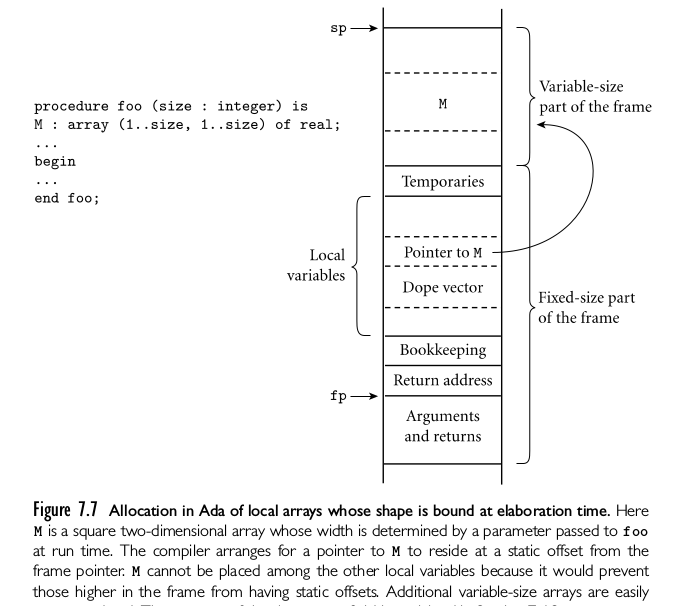
\includegraphics[width=.9\linewidth]{adaarreglo.png}

\subsubsection*{Arreglos}
\label{sec:orgheadline19}
\begin{itemize}
\item Elementos Contiguos
\begin{itemize}
\item Dirigido por Columnas - solo en \textbf{Fortrand}
\item Dirigido por filas
\begin{itemize}
\item usada por el resto de lenguajes
\item hace que el \texttt{array [a..b,c..d]} sea igual a \texttt{array [a..b] of array [c..d]}
\end{itemize}
\end{itemize}
\end{itemize}

\subsubsection*{Arreglos}
\label{sec:orgheadline20}

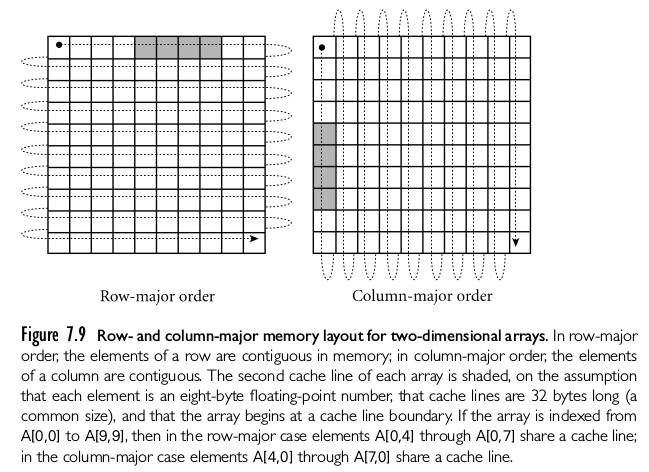
\includegraphics[width=.9\linewidth]{rowcolumnmajor.png}

\subsubsection*{Arreglos}
\label{sec:orgheadline21}

\begin{itemize}
\item \textbf{Dos estrategias para arreglos}
\begin{itemize}
\item Elementos continuos
\item punteros de filas
\end{itemize}
\item \textbf{Punteros de Filas}
\begin{itemize}
\item una opcion en \textbf{C}
\item permite a las filas colocarse en cualquier parte de la memoria
\item bueno para matrices cuando las filas son de diferente longitud
\begin{itemize}
\item ejemplo arreglo de strings
\end{itemize}
\item requiere espacio para los punteros
\end{itemize}
\end{itemize}

\subsubsection*{Arreglos}
\label{sec:orgheadline22}

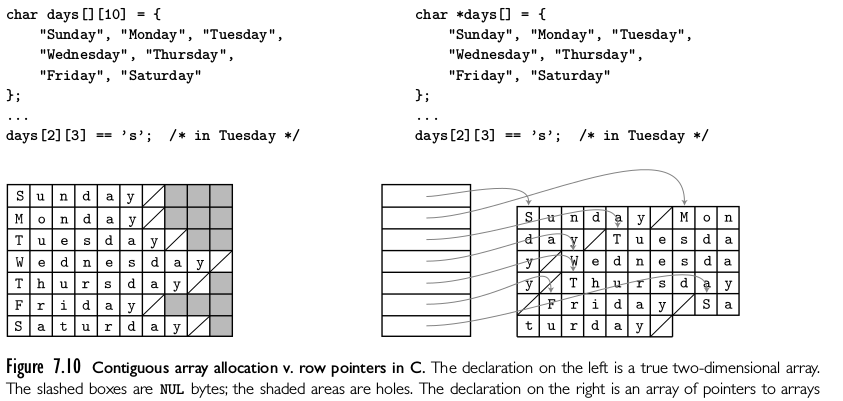
\includegraphics[width=.9\linewidth]{arraypontrowc.png}

\subsubsection*{Inicialización de Arreglos}
\label{sec:orgheadline23}
\begin{itemize}
\item Algunos Lenguajes permiten inicialización en el tiempo de
alojamiento.
\begin{itemize}
\item ejemplo de \textbf{C}, \textbf{C++}, \textbf{Java}, \textbf{C\#}
\begin{itemize}
\item \texttt{int list [] = \{4, 5, 7, 83\}}
\end{itemize}
\item cadena de caracteres en \textbf{C} y \textbf{C++}
\begin{itemize}
\item \texttt{char name [] = "freddie";}
\end{itemize}
\item Array of strings en \textbf{C} and \textbf{C++}
\begin{itemize}
\item \texttt{char *names [] = \{"bob", "jake", "Joe"\};}
\end{itemize}
\item \textbf{Java} 
\begin{itemize}
\item \texttt{String[] names = \{"Bob", "Jake", "Joe"\};}
\end{itemize}
\end{itemize}
\end{itemize}

\subsubsection*{Operaciones de Arreglos}
\label{sec:orgheadline24}
\begin{itemize}
\item \textbf{APL} provee el mas poderoso conjunto de operadores para procesar
vectores y matrices y operaciones unarias (por ejemplo revertir
elementos de una columna)
\item \textbf{Ada} permite asignación de arreglos y concatenación
\item \textbf{Fortran} provee operaciones \emph{elementales} a causa de que son entre
pares de elementos del arreglo
\begin{itemize}
\item Por ejemplo, el operador + entre dos arreglos resulta en un
arreglo con la suma de los pares de elementos de los dos arreglos.
\end{itemize}
\end{itemize}

\subsubsection*{Arreglos}
\label{sec:orgheadline25}
\begin{itemize}
\item Ejemplo \texttt{A : array [L1..U1] of array [L2::U2] of array [L3..U3] of elem;}
\begin{itemize}
\item \(D1 = U1 - L1 + 1\)
\item \(D2 = U2 - L2 + 1\)
\item \(D3 = U3 - L3 + 1\)
\item \(S3 =\) tamaño de \texttt{elem}
\item \(S2 = D3 * S3\)
\item \(S1 = D2 * S2\)
\end{itemize}
\end{itemize}

\(A(i,j,k) =\) \texttt{address of A} \(+ (i * S1) + (j * S2) + (k * S3)  -
[(L1 * S1) + (L2 * S2) + (L3 * S3)]\)


\subsubsection*{Slices}
\label{sec:orgheadline26}
\begin{itemize}
\item Una \emph{porción} (slice) de un arreglo es una subestructura de un
arreglo; un mecanismo de referenciación.
\item Los \emph{Slices} son útilies en lenguages que tienen operaciones sobre
arreglos (APL, FORTRAN etc).
\end{itemize}

\subsubsection*{Slices}
\label{sec:orgheadline27}

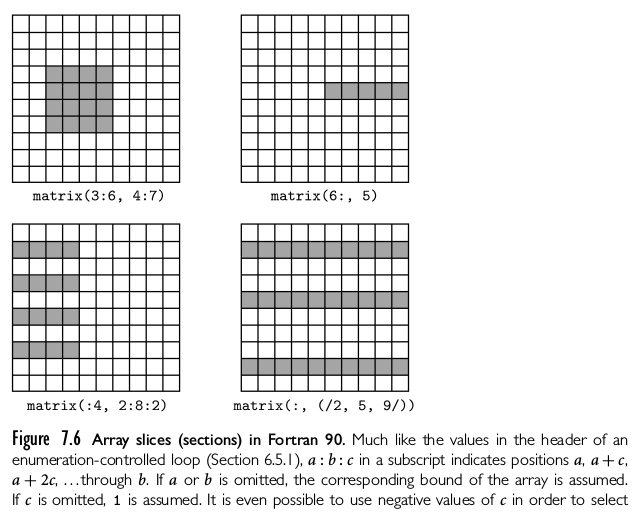
\includegraphics[width=.9\linewidth]{slicesfort.png}

\subsubsection*{Descriptores en Tiempo de Compilación}
\label{sec:orgheadline28}

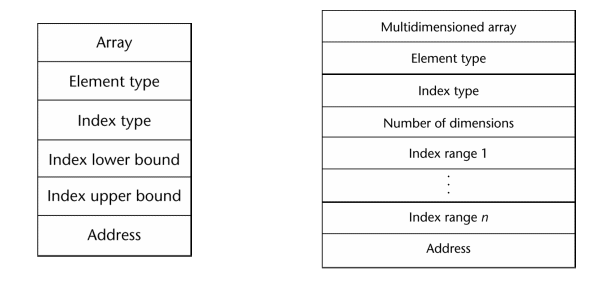
\includegraphics[width=.9\linewidth]{descriptoresarray.png}

\subsubsection*{Arreglos Asociativos}
\label{sec:orgheadline29}
\begin{itemize}
\item Un \emph{arreglo asociativo} es una colección no ordenada de elementos de
datos que son indexados por un numero igual de valores llamados
\emph{claves} (keys)
\begin{itemize}
\item claves definidas por el usuario deben ser almacenadas
\end{itemize}
\item Ahora llamados \emph{Diccionarios}
\item en \textbf{PERL}
\begin{itemize}
\item Nombres comenzando con \texttt{\%}; literales son delimitados con
paréntesis
\begin{itemize}
\item \texttt{\%hi\_temps} = ("Mon" => 77, "Tue" => 79, "Wed" => 65, \ldots{} ),
\end{itemize}
\item Para acceder se usan llaves y claves:
\begin{itemize}
\item \texttt{\%hi\_temps\{"wed"\} = 83;}
\end{itemize}
\item Los elementos pueden ser removidos con \texttt{delete}
\begin{itemize}
\item \texttt{delete \%hi\_temps\{"Tue"\}}
\end{itemize}
\end{itemize}
\end{itemize}


\subsection*{Strings}
\label{sec:orgheadline31}
\begin{itemize}
\item \emph{Strings} son en realidad arreglos de caracteres
\item Son frecuentemente casos especiales, para darles flexibilidad (como
polimorfismo y tamaño dinámico) que no es disponible para arreglos
en general
\begin{itemize}
\item Es mas facil proveer estas cosas para \emph{strings} que para arreglos
en general porque los \emph{strings} son de una dimensión y no circulares.
\end{itemize}
\end{itemize}

\subsection*{Tipo Registros}
\label{sec:orgheadline40}
\begin{itemize}
\item Un registro es un conjunto posiblemente heterogeneo de elementos de
datos en el cual los elementos individuales son identificados por su nombre
\item Cuestiones de Diseño
\begin{itemize}
\item ¿Cual es la sintaxis para referenciar los campos?
\item ¿Son permitidas las referencias elípticas?
\end{itemize}
\end{itemize}

\subsubsection*{Tipo Registros}
\label{sec:orgheadline32}
\begin{itemize}
\item Cobol
\end{itemize}
\begin{verbatim}
01 EMPLOYEE-RECORD.
   02 EMPLOYEE-NAME.
      05 FIRST    PICTURE IS x(20).
      05 MIDDLE   PICTURE IS x(10).
      05 LAST     PICTURE IS x(20).
   02 HOURLY-RATE PICTURE IS 99v99.
\end{verbatim}
\begin{itemize}
\item Ada
\end{itemize}
\begin{verbatim}
type Employee_Name_Type is record
   First : String (1..20);
   Middle : String (1..10);
   Last : String (1..20);
end record;
type Employee_Record_Type is record
   Employee_Name: Employee_Name_Type;
   Hourly_Rate: Float;
end record;
Employee_Record: Employee_Record_Type;
\end{verbatim}

\subsubsection*{Registros}
\label{sec:orgheadline33}
\begin{itemize}
\item Referencia a los campos
\begin{itemize}
\item \textbf{COBOL} \texttt{field\_name OF record\_name\_1 OF ... OF record\_name\_n}
\item Otros (notación con punto) \texttt{record\_name\_1.record\_name\_2. ... record\_name\_n.field\_name}
\end{itemize}
\item Referencias completamente calificadas: debe incluir todo el camino
de nombres de registros.
\item Referencia elíptica: permite no especificar nombres intermedios
siempre que la referencia sea no ambigua. Ej: \texttt{FIRST OF EMP-REC} en \textbf{COBOL}
\end{itemize}

\subsubsection*{Operaciónes de Registros}
\label{sec:orgheadline34}
\begin{itemize}
\item La asignación es muy común si los tipos son identicos
\item \textbf{Ada} permite comparación de registros
\item Los registros de \textbf{Ada} pueden ser inicializados con conjunto de literales
\item \textbf{COBOL} provee \texttt{MOVE CORRESPONDING}
\begin{itemize}
\item copia un campo de un registro origen al correspondiente campo en
el registro destino.
\end{itemize}
\end{itemize}

\subsubsection*{Comparación con Arreglos}
\label{sec:orgheadline35}
\begin{itemize}
\item Tiene un diseño directo y seguro
\item Son usados cuando el agrupamiento de datos es heterogeneo
\item El acceso es mucho mas rápido que en arreglos porque el acceso a los
nombres de los campos es estático
\end{itemize}

\subsubsection*{Implementación de Registros}
\label{sec:orgheadline36}

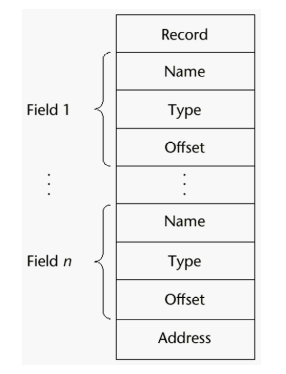
\includegraphics[width=.9\linewidth]{implementregistros.png}

Un desplazamiento de dirección relativo al comienzo del registro es
asociado con cada campo.

\subsubsection*{Tipo Uniones}
\label{sec:orgheadline37}
\begin{itemize}
\item Una \emph{Union} es un tipo a cuyas variables se les permite
almacenar diferentes valores de tipo (estructura) en diferentes tiempos durantes
la ejecución.
\item Cuestiones de Diseño
\begin{itemize}
\item ¿Debería requerirse chequeo de tipos?
\item ¿Deberían incluirse como tipos particulares de Registros?
\end{itemize}
\item \textbf{Fortran}, \textbf{C}, y \textbf{C++} provee constructores de \emph{Union} sin soporte
para chequeo de tipos se llaman \emph{uniones libres}
\item Chequeo de tipos en \emph{Uniones} requieren que se incluya un indicador
de tipo llamado \emph{discriminante}
\begin{itemize}
\item soportado por \textbf{Ada}
\end{itemize}
\end{itemize}


\subsubsection*{tipo Union de Ada}
\label{sec:orgheadline38}
\begin{verbatim}
type Shape is (Circle, Triangle, Rectangle);
type Colors is (Red, Green, Blue);
type Figure (Form: Shape) is record
  Filled: Boolean;
  Color: Colors;
  case Form is 
      When Circle => Diameter : Float;
      When Triangle => 
             LeftSide, Rightside: Integer;
             Angle: Float;
      when Rectangle => Side1,Side2: Integer;
  end case;
end record;
\end{verbatim}
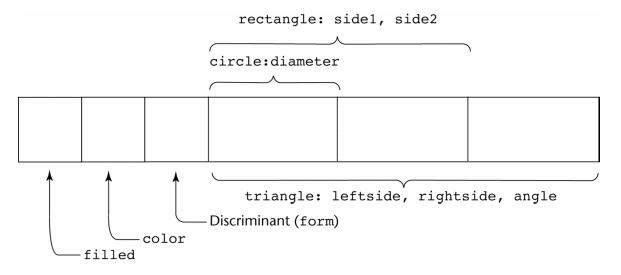
\includegraphics[width=.9\linewidth]{adaunion.png}

\subsubsection*{Evaluación de Uniones}
\label{sec:orgheadline39}
\begin{itemize}
\item también llamados registros variantes
\item Es una construcción potencialmente insegura
\begin{itemize}
\item no permite chequeo de tipos o es muy caro
\end{itemize}
\item \textbf{Java} y \textbf{C\#} no soportan uniones
\begin{itemize}
\item Como reflejo de la creciente preocupación por la seguridad en los lenguajes de programación
\end{itemize}
\item La falta de discriminante (tag) significa que uno no sabe lo que hay almacenado
\item La posibilidad de cambiar el discriminante permite acceder a campos erroneamente
\end{itemize}

\subsection*{Punteros y Tipos Recursivos}
\label{sec:orgheadline46}

\subsubsection*{Tipo Punteros}
\label{sec:orgheadline41}
\begin{itemize}
\item Los Punteros sirven para dos propósitos:
\begin{itemize}
\item acceso eficiente (y a veces intuitivo) a objetos muy elaborados
(como en \textbf{C})
\item creación dinámica de estructuras ligadas, en conjunción con
administración de memoria \emph{heap}
\end{itemize}
\item Varios lenguajes (e.g. \textbf{Pascal} ) restringen los punteros para
acceder a cosas en el \emph{heap}
\item Los punteros son usados en un modo \emph{por valor} de las variables
\begin{itemize}
\item No se necesitan como modo \emph{por referencia}
\end{itemize}
\end{itemize}

\subsubsection*{Punteros y Tipos Recursivos}
\label{sec:orgheadline42}

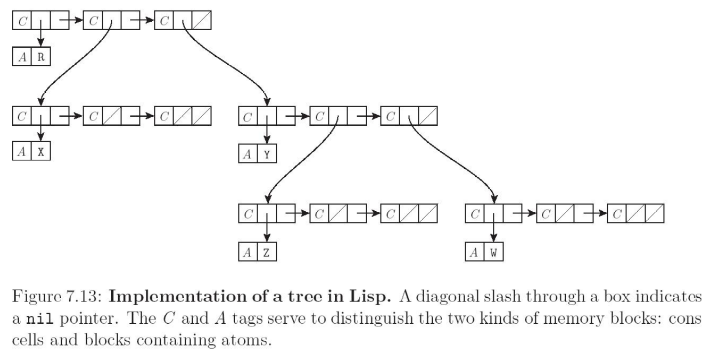
\includegraphics[width=.9\linewidth]{lisppunt.png}

\subsubsection*{Punteros y Tipos Recursivos}
\label{sec:orgheadline43}
\begin{itemize}
\item \textbf{C} punteros y arreglos
\begin{itemize}
\item \texttt{int *a == int a[]}
\item \textasciitilde{}int **a == int *a[]
\end{itemize}
\item Las equivalencias no siempre ocurren
\begin{itemize}
\item Especificamente, una declaración aloja un arreglo si se especifica
un tamaño para la primera dimensión
\item en caso contrario aloja un puntero
\begin{itemize}
\item \texttt{int **a, int *a[]} puntero a puntero a int
\item \texttt{int *a[n]},  arreglo de \emph{n} elementos de punteros
\item \texttt{int a[n][m]} arreglo de dos dimensiones
\end{itemize}
\end{itemize}
\end{itemize}

\subsubsection*{Punteros y Tipos Recursivos}
\label{sec:orgheadline44}
\begin{itemize}
\item El compilador tiene que ser capaz de establecer el tamaño de las
cosas apuntadas por los punteros
\begin{itemize}
\item Por lo tanto las siguientes no son válidas:
\begin{itemize}
\item \texttt{int a[][]} mal
\item \texttt{int (*a)[]} mal
\end{itemize}
\item regla de declaración de \textbf{C}: lee a la derecha tanto como puede
(sujeto a paréntesis), luego a la izquierda, y luego sube de nivel
y repite.
\begin{itemize}
\item \texttt{int *a[n]} arreglo de \emph{n} elementos de punteros a enteros
\item \texttt{int (*a)[n]} puntero a un arreglo de \emph{n} elementos de enteros
\end{itemize}
\end{itemize}
\end{itemize}

\subsubsection*{Punteros y Tipos Recursivos}
\label{sec:orgheadline45}
\begin{itemize}
\item Los problemas con punteros \emph{cogados} se deben a:
\begin{itemize}
\item desalojo explícito de objetos del \emph{heap}
\begin{itemize}
\item solo en lenguajes que tienen explícito desalojo
\end{itemize}
\item desalojo implícito de objetos elaborados
\end{itemize}
\item Dos mecanismos de implementación para atrapar punteros \emph{colgados}
\begin{itemize}
\item \emph{Tombstones} lapidas
\item \emph{Locks and Keys} llaves y cerraduras
\end{itemize}
\end{itemize}

\subsection*{Listas}
\label{sec:orgheadline47}
\begin{itemize}
\item Una \emph{Lista} es definida recursivamente ya sea como una lista vacía o
un par consistente de un objeto (que puede ser una lista o un átomo)
y otra lista (mas corta)
\begin{itemize}
\item Las \emph{Listas} son ideales para programar en lenguajes lógicos y funcionales
\begin{itemize}
\item En \textbf{Lisp} de hecho un programa \emph{es} una lista, y puede
extenderse a si mismo para construir una lista y ejecutarla
\end{itemize}
\item Las \emph{Listas} pueden usarse en programas imperativos.
\end{itemize}
\end{itemize}

\subsection*{Archivos y Entrada/Salida}
\label{sec:orgheadline48}
\begin{itemize}
\item Entrada/Salida (E/S) facilita al programa a comunicarse con el mundo externo
\begin{itemize}
\item E/S interactiva y E/S con archivos
\end{itemize}
\item Interactivo generalmente implica comunicación con usuarios humanos y
dispositivos físicos
\item Archivos generalmente se refieren a almacenamiento fuera de linea
implementado por el sistema operativo.
\item Archivos pueden ser categorizados en:
\begin{itemize}
\item Temporarios
\item Persistentes
\end{itemize}
\end{itemize}
\end{document}
